\section{Project Scope}

As stated in the literature survey and after discussing with industry experts, the author found many issues that could be addressed when developing this system, but some of those problems, like getting the models well optimised to react to the anomalies, is a complex task to achieve. 
% As this project is done by one developer in less than one year, it won't be possible to create a fully functional monitoring platform like Datadog or New Relic. 
Therefore, the main focus of this project is to create an end-to-end framework which will make the application of machine learning to solve \ac{sre} issues straightforward, so future work can be built upon this project.

\subsection{In-scope} \label{sec:in-scope}
Following are the main focusses of this project.
\begin{itemize}[noitemsep,nolistsep] 
    \item Low overhead data collection pipeline to collect service telemetry.
    \item Loosely coupled architectures, so that all components can be individually deployed.
    \item UI to easily visualize the service topology and identify root causes.
    \item Optimized models that have a small memory footprint and CPU overhead.
    \item Well generalised model which will be able to be deployed with completely new services and will learn to adapt to the new system.
    \item System should adopt to very large systems High Scalability.
    \item Interpretable models.
    \item Easily adaptable.
\end{itemize}


\subsection{Out-scope} \label{sec:out-scope}
Follow will not be covered during this project
\begin{itemize}[noitemsep,nolistsep]
    \item Working outside of Kubernetes eco-system.
    \item Intergrate with websockets.
    \item Acts as a fully functional monitoring system.
    \item Multi-Cluster support
    \item Highly accurate predications of the model.
\end{itemize}

\subsection{Prototype Feature Diagram}
\begin{figure}[H]
    \centering
    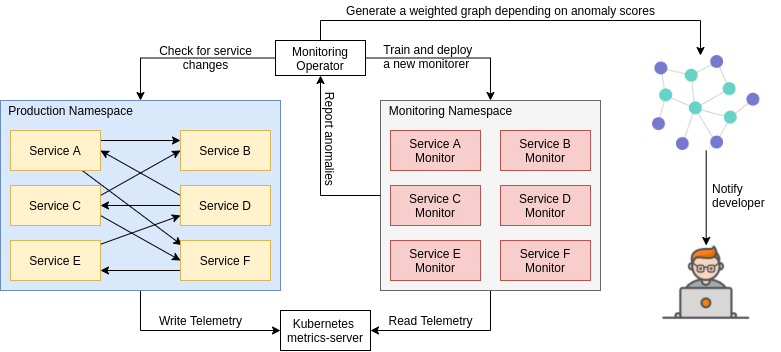
\includegraphics[width=14.9cm]{assets/introduction/High-level-system-diagram.png}
    \caption{Prototype feature diagram (self composed)}
    \label{fig:high-level-diagram}
\end{figure}